\documentclass{beamer}

\usepackage{amsmath}
\usepackage{amssymb}
\usepackage{amsthm}

\title{Proofs in Three Bits of Less}
\author{Jacob Denson}
\institute{University of British Columbia}

\begin{document}

\maketitle

\begin{frame}
    \frametitle{What Are Interactive Proofs?}

    \begin{itemize}
        \item<1-> Like 20 Questions -- the {\bf verifier} asks yes/no questions to a {\bf prover} until they are convinced a proof is correct, or incorrect.

        \item<2-> More versatile than classical proofs -- we can ask questions like
        %
        \begin{center} ``Answer Yes If the n'th bit in the binary encoding of your proof is a 1, else 0''
        \end{center}
        %
        to recover classical proofs.

        \item<3-> We can measure a theorem's difficulty by how many questions it takes for us to become convinced.
    \end{itemize}
\end{frame}

\begin{frame}
    \frametitle{Watch Out For Tricks!}

    The verifier {\it cannot} trust the prover. The could either be making mistakes, or maliciously trying to trick you into thinking the proof is correct! The question
    %
    \begin{center} ``Is your proof correct?'' \end{center}
    %
    Is useless. Questions must be checkable!

    (Origins in Cryptography)
\end{frame}

\begin{frame}
    \frametitle{Completeness and Soundness}

    \begin{columns}

    \column{1\textwidth}
    \begin{center} Classical Proofs have \end{center}
    %
    \begin{itemize}
        \item<1-> {\bf Perfect Completeness}: If a statement is true, there exists a series of answers to the questions we give which will convince us the statement is true.

        \item<2-> {\bf Perfect Soundness}: If a statement is false, {\it no} series of answers to the questions I give will convince me the statement is true. You can't trick me!
    \end{itemize}

    \end{columns}
\end{frame}

\begin{frame}
    \frametitle{The Catch!}

    Proofs of very short statements can be arbitrary long. Very inefficient. Consider the theorem
    %
    \begin{center}
        `` This Theorem Cannot Be Proved In Less Than a Googleplex Symbols ''
    \end{center}
    %
    A 53 character theorem with a HUGE proof.
\end{frame}

\begin{frame}
    \frametitle{Weakening Proof Conditions}

    If we let the questions we ask be randomized, then we can weaken completeness and soundness conditions:
    %
    \begin{itemize}
        \item<2-> {\bf Imperfect Completeness}: If a statement is true, there exists a series of answers to the questions which convince you the truth with probability $\geq 1/2$.

        \item<3-> {\bf Imperfect Soundness}: If a statement is false, {\it every} series of answers to the questions I give will fail to convince me the statement is true with probability $\geq 1 - \varepsilon$. It's unlikely you'll trick me!
    \end{itemize}
\end{frame}

\begin{frame}
    \frametitle{The PCP Theorem}

    \begin{theorem}[1998, Arora, Lund, Motwani, Sudan, Szegedy]
        There exists a universal constant $K$ such that, for any ``feasibly checkable'' mathematical problem, we can check the problem with perfect soundness and imperfect completeness in $K$ questions.
    \end{theorem}

    \begin{theorem}[1997, H\r{a}stad]
        If you only want imperfect completeness, you can set $K = 3$!
    \end{theorem}
\end{frame}

\begin{frame}
    \frametitle{A Practical Application: Bitcoin}

    \begin{itemize}
        \item<1-> Bitcoin is a decentralized currency; there's no bank verifying the correctness of transactions.

        \item<2-> Volunteers known as `miners' verify correctness in huge ledgers in exchange for small amounts of currency.

        \item<3-> The PCP theorem has been proposed as a way to make fraud detection in Bitcoin `scalable' -- in exchange for accidently identifying true claims as false every so often, we only need a constant number of queries to become convinced of a transaction.
    \end{itemize}
\end{frame}

\begin{frame}
    \frametitle{Globalization of Local Properties}
    \begin{itemize}
        \item<1-> We can view a set of questions that convince us of a theorem as an {\it encoding} of the proof of the theorem. The PCP theorem says that local properties can be encoded globally.

        \item<2-> $O(|V|)$ questions to determine if a graph has a 3-coloring. The PCP theorem says we can encode a coloring of a graph in such a way that, if the graph fails to be colorable, it will be displayed globally in the encoding -- we can detect it with $O(1)$ samples.
        %
        \begin{center}
        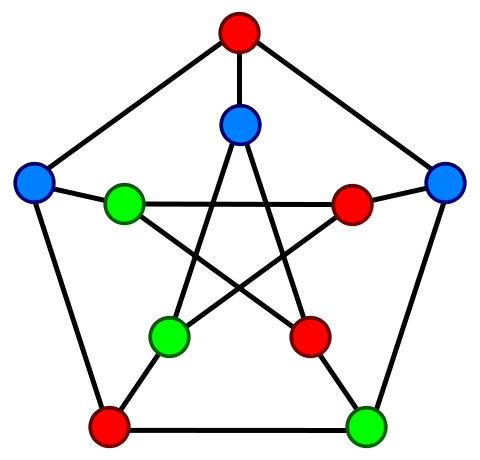
\includegraphics[scale=0.25]{3coloring.jpg}
%        \scalebox{0.5}{\text{https://en.wikipedia.org/wiki/Graph_coloring}}
    \end{center}
    \end{itemize}
\end{frame}

\begin{frame}
    \frametitle{Globalization of Local Properties}

    \begin{itemize}
        \item<1-> We can determine if an integer has 100 prime factors with high probability in three questions!

        \item<2-> We can't determine the factorization, just that the factorization exists.

        \item<3-> Fourier Analysis is useful for globalizing local properties -- $L^\infty$ norm of $f$ is local, but can be controlled by $L^1$ norm of $\hat{f}$, which is a global property.
    \end{itemize}
\end{frame}

\begin{frame}
    \frametitle{Sushi Break + An Analogy}

    \begin{center}
        
\includegraphics[scale=0.4]{sushi.jpg}\\
        \scalebox{0.5}{https://dynermite.wordpress.com/2011/05/04/adorable/}
    \end{center}

    % Put Sushi Picture

    \begin{itemize}
        \item Any questions so far?
    \end{itemize}
\end{frame}

\begin{frame}
    \frametitle{First Example: PCP Checker For Graph Nonisomorphism}

    \begin{itemize}
        \item<1-> Two graphs are isomorphic if they can be obtained from one another by relabeling vertices. We take two graphs $G_0$ and $G_1$ on $n$ vertices, and ask if they are {\it not} isomorphic to each other.

        \item<2-> A proof that two graphs are isomorphic is short -- just give an isomorphism. A proof that two graphs are not isomorphic is {\it very difficult}: check by cases. We give a 1 query proof.
    \end{itemize}

    \begin{center}
        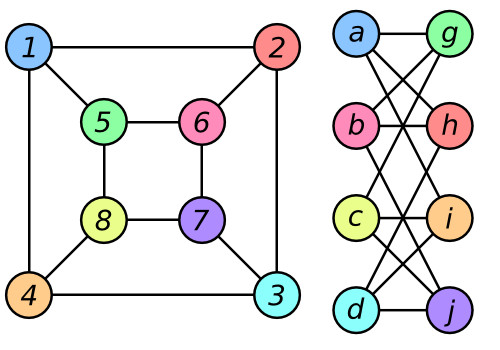
\includegraphics[scale=0.3]{graphisomorphism.jpg}\\
        \scalebox{0.5}{http://proopnarine.files.wordpress.com/2010/02/isomorphic.png}
    \end{center}

    % Put picture of Graph Isomorphism Here
\end{frame}

\begin{frame}
    \frametitle{The Checker}

    \begin{itemize}
        \item<1-> Ask questions of the following variety, for some graph $H$
        %
        \begin{center}
            `` If $H$ is isomorphic to $G_0$, output 0. If $H$ is isomorphic to $G_2$, output 0. Otherwise, output an arbitrary result. ''
        \end{center}
        %
        Note that if $G_0 \cong G_1$, the question doesn't even make sense.

        \item<2-> To obtain a question at random, pick an index $i \in \{ 0, 1 \}$ and a permutation $\pi \in S_n$ uniformly at random. Let $H = \pi(G_i)$. We are convinced of the proof if answer to our question corresponds to the correct answer $H \cong G_i$.

        \item<3-> If $G_0$ {\it is} isomorphic to $G_1$, then $H$ is independent of $i$, so $\mathbf{P}(i = 0 | H) = \mathbf{P}(i = 1 | H) = 1/2$, and so regardless of the answer the prover gives, they have a 50\% chance of getting the answer wrong.
    \end{itemize}

    % Put picture of Graph Isomorphism Here
\end{frame}

\begin{frame}
    \frametitle{But Wait!}

    \begin{itemize}
        \item<1-> How many different questions can we ask? About $O(n!)$. We can view this as an encoding of the graph in $O(n!)$ bits.
        \item<2-> If original graph has $m$ vertices, can be encoded in $O(m)$ bits.
        \item<3-> HUGE increase in size of encoding to obtain globality. The PCP theorem guarantees that we only increase our encoding by $O(n)$. The PCP theorem doesn't apply to the graph nonisomorphism problem because it isn't feasibly checkable -- we only know it to be checkable in exponential time, by cases.
    \end{itemize}
\end{frame}

\begin{frame}
    \frametitle{Local Proofs: The BLR test}

    \begin{itemize}
        \item<1-> Local proofs are a key tool for moving from local properties to global properties. The most important one is the {\bf Blum-Luby-Rosenfeld Test}.

        \item<2-> Answers the question: How many queries does it take to check that $f: \mathbf{F}_2^n \to \mathbf{F}_2$ is linear (Answer: 3).

        \item<3-> Take $X,Y \in \mathbf{F}_2^n$ uniformly at random. We are convinced if
        %
        \[ f(X + Y) = f(X) + f(Y) \]

        \item<4-> Perfect completeness: If $f$ is linear, we are always convinced.
        \item<5-> Local soundness: If $f$ convinces us it is linear with probability $1 - \varepsilon$, there is a linear function $g$ such that $d(f,g) \leq \varepsilon$, where
        %
        \[ d(f,g) = \frac{\{ x \in \mathbf{F}_2^n: f(x) \neq g(x) \}}{2^n} \]
        %
        is the {\bf Hamming distance} between two functions.
    \end{itemize}
\end{frame}

\begin{frame}
    \frametitle{Local Correctibility}

    \begin{itemize}
        \item<1-> Linearity can Fail Locally, but we can cheat.

        \item<2-> Suppose $d(f,g) \leq \varepsilon$. Then $f$ and $g$ agree with a large number of inputs, but differ on a couple of inputs deterministcally.

        \item<3-> Given {\it any x}, can we calculate $g(x)$ using only $f(x)$, even if $f(x) \neq g(x)$?

        \item<4-> Take $Y \in \mathbf{F}_2^n$ uniformly at random. Then $f(x + Y) - f(Y) = g(x
        )$ with probability $\geq 1 - 2 \varepsilon$.

        \item<5-> Even though linearity can fail locally, we can think of $f$ as an encoding of $g$ if it is close enough, so essentially, we can view all functions which are close to linear functions -- we've moved from local error to global error.
    \end{itemize}
\end{frame}

\begin{frame}
    \frametitle{The Big PCP Test: Quadratic Equations}

    \begin{itemize}
        \item<1-> Consider the problem of determining whether a series of quadratic equations over $\mathbf{F}_2$ is solvable, e.g.
        %
        \[ x_1^2 + x_2x_3 + x_4^2 = 1\ \ \ \ \ x_5^2 + x_2x_6 + x_1^2 = 0 \]

        \item<2-> Since $x_i^2 = x_i$, we can assume all monomials have degree two.

        \item<3-> Since this problem is {\bf NP Hard}, all feasibly checkable problems are reducible to this problem, so a PCP theorem for this problem gives a PCP checker for all problems. However, we won't only use a linear number of questions.
    \end{itemize}
\end{frame}

\begin{frame}
    \frametitle{The Test}

    \begin{itemize}
        \item<1-> If someone has a solution $x$, our checker will ask the following two kinds of questions:
        %
        \begin{itemize}
            \item<2-> `` For some subset $S \subset [n]$ of indices, what is $\sum_{i \in S} x_i$. ''
            \item<3-> `` For some subset $S \subset [n] \times [n]$, what is $\sum_{(i,j) \in S} x_ix_j$. ''
        \end{itemize}
        %
        \item<4-> These values will enable us to check quadratic equations in very few queries.
    \end{itemize}
\end{frame}

\begin{frame}
    \frametitle{The Test}

    \begin{itemize}
            \item<1-> We start by picking subsets $S$ and $T$, $S'$, $T'$, uniformly at random, and ask if
        %
        \[ \sum_{i \in S} x_i + \sum_{i \in T} x_i = \sum_{i \in S \Delta T} x_i \]
        %
        \[ \sum_{(i,j) \in S'} x_ix_j + \sum_{(i,j) \in T'} x_ix_j = \sum_{(i,j) \in S' \Delta J'} x_ix_j \]

        \item<2-> Note this is the BLR test if the maps $S \mapsto \sum x_i$ and $S' \mapsto \sum x_ix_j$ are {\it linear}, where we view $2^{[n]}$ and $2^{[n] \times [n]}$ as vector spaces over $\mathbf{F}_2$ with $S + T := S \Delta T$.

        \item<3-> If a particular answer passes with high probability, then it is close to an {\it actual} linear operator on $2^{[n]}$ and $2^{[n] \times [n]}$, and all such linear operators are given by some $x$. Local correction means we can calculate values of a real $x$.
    \end{itemize}
\end{frame}

\begin{frame}
    \frametitle{The Test}

    \begin{itemize}
        \item<1-> If the last questions passed, we can assume we can calculate the sums for an {\it actual} $x$, rather than the answers the prover is giving to us, which might be false.

        \item<2-> If the quadratic equations are
        %
        \[ \sum_{(i,j) \in T_k} x_ix_j = b_k \]
        %
        for some $k \in \{ 1, \dots, m \}$, then pick a random subset $S = \{ i_1, \dots, i_l \} \subset [m]$, set $T = T_{i_1} \Delta \dots \Delta T_{i_l}$ and test if
        %
        \[ \sum_{(i,j) \in T} x_ix_j = \sum_{i \in T} b_i \]

        \item <3-> If a single equation fails to be satisfied, then the linear function on left doesn't equal the linear function on right, and therefore disagrees on half the inputs. Fails half the time.
    \end{itemize}
\end{frame}

\begin{frame}
    \frametitle{Why Do We Care? Complexity Theory}

    \begin{itemize}
        \item<1-> A problem is in {\bf NP} if a solution can be checked in polynomial time, and in {\bf P} if the solution can be found in polynomial time.

        \item<2-> Determining a three coloring in a graph is hard, but I can check a given coloring is a three coloring very quickly -- $O(n^2)$ in the number of vertices, a polynomial bound.

        \item<3-> It is an open problem whether we can factor an integer fast -- i.e. is integer factorization in ${\bf P}$. However, if you give me a set of factors, I can determine if they are the factors of a particular integer just by multiplying the integers together -- simple!

        \item<4-> The current state of the art factorization algorithm runs in time proportional to
        %
        \[ O \left( \exp \sqrt[3]{\frac{64}{9} n (\log n)^2} \right) \]
        %
        where $n$ is the bit number to represent the number we factor.
    \end{itemize}
\end{frame}

\begin{frame}
    \frametitle{Cook's Theorem}

    \begin{theorem}[Canada, Cook, 1971; USSR, Levin, 1969]
        There exists problems, known as {\bf NP Hard} problems, on which every feasibly checkable problem, known as an {\bf NP problem}, can be encoded in the NP hard problem in polynomial time.
    \end{theorem}

    \begin{itemize}
        \item<2-> If an {\bf NP} hard problem has a polynomial time solution, {\it all} {\bf NP} problems are solvable in polynomial time, so {\bf NP = P}. Since most people believe {\bf NP} $\neq$ {\bf P}, {\bf NP} hard problems are {\it hard} to solve efficiently.

        \item<3-> The first {\bf NP} hard problem discovered was 3-SAT. Given a logical formula, e.g.
        %
        \[ (x_1 \vee x_2 \vee x_4) \wedge (x_5 \vee x_1 \vee x_7) \wedge (x_1 \vee x_2 \vee x_4) \]
        %
        a conjunction of three variable disjunctions, can we give variables truth values to make the statement true?
    \end{itemize}
\end{frame}

\begin{frame}
    \frametitle{Approximation Algorithms}

    \begin{itemize}
        \item<1-> {\bf NP} hard problems cannot be solved efficiently, but maybe we can `approximately' solve them efficiently.

        \item<2-> Rather than asking if a formula is satisfiable, turn into an optimization problem, {\it how many} clauses can we satisfy.

        \item<3-> For $A < 1$, an $A$ approximation algorithm is an efficient algorithm such that if it is possible to satisfy a fraction $B$ of the clauses, we find an assignment satisfying $AB$ clauses.

        \item<4-> A random assignment satisfies $7/8$ of the clauses, and we can derandomize to get $7/8$ approximation algorithm.
    \end{itemize}
\end{frame}

\begin{frame}
    \frametitle{Generalizing Cook's Lemma}

    \begin{itemize}
        \item<1-> Is there a limit to how well we can approximate a problem? Maybe we can find a $1 - \varepsilon$ approximation for every $\varepsilon$ (true for certain problems, like knapsack).

        \item<2-> Every problem can be reduced to 3SAT, but the solutions aren't `globally' separated. A solution to 3SAT can fail at a single clause, but satisfy almost all clauses.

        \item<3-> Each possible random query in PCP theorem can be viewed as a clause of a 3SAT problem, that separates incorrect solutions ($\leq 1/2$ clauses satisfiable), from correct clauses ($1 - \varepsilon$ of clauses solvable).

        \item<4-> H\r{a}stad used this to show that for any $\varepsilon > 0$, if there is a $7/8 + \varepsilon$ approximation algorithm for $3SAT$, then $\mathbf{P} = \mathbf{NP}$. Thus the $7/8$ approximation given before is best possible.
    \end{itemize}
\end{frame}

\begin{frame}
    \frametitle{Where to Go From Here?}

    \begin{itemize}
        \item<1-> The rest of PCP theorem proof involves interesting combinatorial techniques (e.g. expander graphs).

        \item<2-> Modern day research in approximability involves deriving checkable proofs for various problems -- interesting probability theory (unique games conjecture, majority is stablest (2007), hypercontractivity, discrete log sobolev inequalities, etc).

        \item<3-> Learning Theory -- Connections between problems that have quick checkable proofs and learning models that are easy to learn. We saw linear functions are easy to learn.

        \item<4-> Connections to Additive Combinatorics: Gower's Inverse Conjecture, constructions of PCPs.

        \item<5-> References:
        \begin{itemize}
            \item Arora, Barak; Computational Complexity.
            \item O' Donell; Analysis of Boolean Functions.
            \item Bellare, Coppersmith, H\r{a}stad, Kiwi, Sudan; Linearity Testing in Characteristic Two.
        \end{itemize}
    \end{itemize}
\end{frame}

\end{document}